\documentclass[25pt,a0paper,blockverticalspace=20mm]{tikzposter}

\usepackage[american]{babel}
\usepackage[utf8]{inputenc}
\usepackage[T1]{fontenc}
\usepackage{amsmath,amssymb}
\usepackage{tikzsymbols}
\usepackage{wrapfig,graphicx}
\usepackage{tikz}
\usepackage{url}

\usetikzlibrary{matrix,arrows,arrows.meta,positioning}
\tikzset{>/.tip={Computer Modern Rightarrow[scale=2,line width=1pt]}}
\tikzset{|/.tip={Bar[scale=2,line width=1pt]}}
\tikzset{c_/.tip={Hooks[scale=2,line width=1pt,right]}}
\tikzset{c^/.tip={Hooks[scale=2,line width=1pt,left]}}

\def\F {\ensuremath{\mathbb{F}}}
\def\Z {\ensuremath{\mathbb{Z}}}
\def\O {\ensuremath{\mathcal{O}}}
\def\from {\,:\,}
\renewcommand{\mod}[1]{\ensuremath{\ (\mathrm{mod}\ #1)}}

\DeclareMathOperator{\End}{End}
\DeclareMathOperator{\Ker}{Ker}

\renewcommand{\paragraph}[1]{\smallskip\textbf{#1.}}
\newcommand{\secblock}[1]{\block[]{}{\huge\sc #1}}

\title{Isogeny-based cryptography in Julia/Nemo : a case study}
\author{Jean Kieffer\footnotemark[1], Luca De Feo\footnotemark[2]}\institute{\footnotemark[1]\'Ecole normale sup\'erieure de Paris
  \footnotemark[2]Université
  de Versailles -- Saint-Quentin-en-Yvelines}

\usetheme{Envelope}

%\definecolorpalette{UVSQ}{
%    \definecolor{colorOne}{RGB}{255,255,255}
%    \definecolor{colorTwo}{RGB}{0,146,187}
%    %\definecolor{colorThree}{RGB}{119,173,28}
%}
%\colorlet{alert}{red}
%\usecolorstyle{Spain}
%
%\definetitlestyle{WLogos}{
%    width=\paperwidth, roundedcorners=0, linewidth=0pt, innersep=1.5cm,
%    titletotopverticalspace=0mm, titletoblockverticalspace=20mm,
%    titlegraphictotitledistance=10pt, titletextscale=1
%}{
%  \draw[draw=none, bottom color=titlebgcolor, top color=framecolor,opacity=0.9]%
%  (\titleposleft,\titleposbottom) rectangle (\titleposright,\titlepostop); %
% \draw
%   (\titleposleft,0.75*\titlepostop+0.25*\titleposbottom)
%   node[anchor=west]{\includegraphics[width=15em]{uvsq-logo-cmjn}}
%   (\titleposright-1em,0.75\titlepostop+0.25*\titleposbottom)
%   node[anchor=east]{\includegraphics[width=15em]{western}}
%   (\titleposleft+1em,\titleposbottom+1em)
%   node[anchor=south west]{\includegraphics[height=5em]{Anssi}}
%   (\titleposright-1em,\titleposbottom+1em)
%   node[anchor=south east]{\includegraphics[height=5em]{Anssi}};
%
%}
%\usetitlestyle{WLogos}

\pgfmathsetseed{\number\pdfrandomseed}
%\definebackgroundstyle{FancyBack}{
%  \draw[opacity=0.2] (0,0) 
%  node[rotate={random(0,359)}]{}
  %\includegraphics[height=\textheight]{Anssi}};
%}
%\usebackgroundstyle{FancyBack} causes problems

\begin{document}
\maketitle

\begin{columns}

\column{0.333}

%First column

\block{Elliptic curves over $\F_p$}{
Let $p$ be a prime number. An \emph{elliptic curve} $E/\F_p$ is a smooth algebraic curve of genus one defined over $\F_p$, with a rational point $\O_E$. Examples :
\begin{itemize}
\item \emph{Weierstrass equations} : $\O_E$ at infinity,
$$E\ :\ y^2 = x^3 + ax + b,\quad 4a^3-27b^2\neq 0$$
\item \emph{Montgomery equations} : $\O_E$ at infinity,
$$E\ :\ B y^2 = x^3 + Ax^2 + x,\quad B(A^2-4)\neq 0.$$

\end{itemize}

$E(\F_{p^r})$ is an abelian group with neutral element $\O_E$ : provides lots of algebraic groups (cf. ECM for factoring, DLP on elliptic curves)

\paragraph{Isogenies}
An \emph{isogeny} between elliptic curves is a nonzero rational map
$$ \phi\from E\to E'$$
that is also a morphism of abelian groups. Call \emph{$\ell$-isogeny} an isogeny of degree $\ell$.
}

\block{Isogeny graphs}{
Define \emph{isogeny graphs} as follows :
\begin{itemize}
\item Vertices are elliptic curves over $\F_p$ up to isomorphism,
\item Edges are isogenies linking them.
\end{itemize}

For ordinary elliptic curves, connected components of isogeny graphs usually have the following shape \cite{Kohel}:

%Picture
\vspace{5cm}

\paragraph{Action of a class group}
Let $E/\F_p$ be an ordinary elliptic curve. The ring $\End(E)$ is isomorphic to an order $\O$ in a quadratic imaginary field. The class group of $\O$ acts simply transitively on the set of elliptic curves with endomorphism ring $\O$.

\paragraph{Representation of ideals} Let $\mathfrak{l}$ be an ideal in $\O$ of prime norm $\ell$. Let $\pi\in\O$ be the Frobenius endomorphism. Then 
$$\O/\mathfrak{l} \simeq \Z/\ell\Z.$$
Call $v = \pi \mod{\mathfrak{l}}$ a \emph{Frobenius eigenvalue}. The ideal $\mathfrak{l}$ is now determined by $(\ell, v)$, and acts as an $\ell$-isogeny.
}

\block{Cryptosystem construction}{
\paragraph{General setting}
Let $G$ be a finite abelian group, and let $X$ be a set with a fixed point $x_0$ on which $G$ acts simply transitively. Define an analogue of the Diffie--Hellman key exchange protocol \cite{Couv}:

\begin{center}
 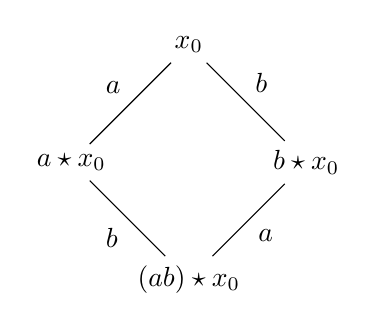
\begin{tikzpicture}[node distance=6em]
  \node(ab){$(ab) \star x_0$};
  \node(a)[above left of=ab]{$a\star x_0$};
  \node(b)[above right of=ab]{$b\star x_0$};
  \node(id)[above left of=b]{$x_0$};
  \draw[]
   (ab) edge[auto] node{$b$} (a)
   (b) edge[auto] node{$a$} (ab)
   (a) edge[auto] node{$a$} (id)
   (id) edge[auto] node{$b$} (b);
 \end{tikzpicture}
\end{center}

Use this general construction for the action above \cite{RoSt}.

\paragraph{Random sampling}
For cryptographic-size parameters, the structure of the class group is unknown. Use a random walk in the isogeny graph instead : under the GRH, it comes close to the uniform distribution \cite{GRH}.

\paragraph{Goal} For various primes $\ell$, compute efficiently the action of an ideal of prime norm $(\ell, v)$ on a curve $E$ : that is, $\ell$-isogenies with domain $E$.
}

%Second column

\column{0.333}

\block{Isogeny computations}{
\paragraph{Modular polynomials}
The modular polynomial $\Phi_\ell(X, Y)$ has the following property : the roots of
$$\Phi_\ell(j(E), Y)$$
in $\F_p$ classify the neighbors of $E$ in the $\ell$-isogeny graph.

\paragraph{Two roots} In our setting we find two neighbors. To choose the one corresponding to an ideal $(\ell, v)$, compute the kernel of this isogeny : it is a $\Z/\ell\Z$-vector space of dimension one stable under the Frobenius endomorphism of $E$. Its eigenvalue must be $v$.
}

\block{Finding the kernel}{
\paragraph{Bostan--Morain--Salvy--Schost~\cite{BMSS}} Suppose $\ell$ is odd. A $\ell$-isogeny $\phi$ may be written
$$\phi(x, y) = \left(\frac{N(x)}{D^2(x)},\ cy \left( \frac{N}{D^2}\right)'(x) \right)$$
The polynomial $D$ defines $\Ker(\phi)$. The rational fraction
$$U(X) = \frac{N(1/X)}{D(1/X)}$$
satisfies a differential equation that is solved efficiently with a Newton iteration.
At the end, recover the polynomial $D$ using the Berlekamp--Massey rational reconstruction algorithm.

Remark that we know of no quasi-optimal algorithm when low characteristic prevents from using BMSS.

\paragraph{Computing the eigenvalue} In the ring $\F_p[x, y]/(D, E)$, where $E$ denotes the curve equation, check the equality
$$[v] (x, y) = (x^p, y^p).$$
LHS is scalar multiplication on the elliptic curve.
}

\block{Cost analysis}{
\paragraph{Costly steps} Both finding roots of modular polynomials, using the Cantor--Zassenhaus algorithm, and computing the eigenvalue involve computing
$$X^p \mod{Q}$$
where $Q$ has degree $\ell$. This is the costly operation both in theory and practice. 

\paragraph{Timing results} The following measurements for this operation were made on a 3.20GHz Intel Xeon workstation, using the Nemo~\cite{Nemo}, Sage~\cite{Sage} and PARI~\cite{PARI} built-ins. Sage relies on PARI, GMP~\cite{GMP} and NTL~\cite{NTL} here.

%Graph
\vspace{5cm}

\paragraph{Total cost} Aiming for reasonable security, we obtain a complete walk in the isogeny graph in approximately 7 minutes, with 20 seconds spent on each of the largest primes.
}

%Third column

\column{0.333}

\block{Speeding computations with torsion points}{
\paragraph{An alternative method}
Supopse $E$ has points of order $\ell$
defined over $\F_p$. Proceed as follows :
\begin{itemize}
\item Choose a random point $P$ in $E(\F_p)$,
\item $Q \gets [C/\ell]P$ until $Q\neq \O_E$, where $C = \#E(\F_p)$
\item Use V\'elu's formul\ae\ to find the isogenous curve.
\end{itemize}

\paragraph{Cost analysis} If $\ell$ is not too large, the scalar multiplication dominates. Using Montgomery curves here brings practical improvements. We implemented our own Montgomery and generic arithmetic in Nemo, and used built-in scalar multiplication in Sage.

\paragraph{Timing results} Again the workstation runs a 3.20GHz Intel Xeon.

%graph
\vspace{5cm}
}

%\block{Implementation}{
%
%}

\block{Parameter determination}{
\paragraph{Exploiting the speed-up} The goal is now to find an $E_0/\F_p$ such that many small primes divide $\# E_0(\F_{p^d})$ for small $d$. We use an exhaustive search strategy :
\begin{itemize}
\item Generate candidates using a simple equation of a certain modular curve, for example the hyperelliptic $X_0(30)$.
\item Test if rational $\ell$-torsion is present for some small primes $\ell$, computing Frobenius eigenvalues as before.
\item If these tests passed, compute the cardinality in full using the Schoof--Atkin--Elkies algorithm and keep the best curves.
\end{itemize}
This method is designed to balance the costs, as computing the cardinality is time-consuming, and is much more efficient than using higher-level modular equations.

\paragraph{Results} We managed to reach 20 primes dividing $\#E(\F_{p^d})$ for $d\leq 10$.
}

\block{\refname}{
	\small
    \renewcommand*{\refname}{\vspace{-1em}}
    \bibliographystyle{plain}
    \bibliography{bibposter}
}

\end{columns}

\end{document}
